\chapter{La catalyse}\label{ch:g12:catalysis}

Un flacon d'eau oxygénée reste des mois dans l'armoire de la salle de
bains sans changer. Versée sur un genou écorché, elle mousse aussitôt~:
quelque chose dans le sang la fait se décomposer en quelques secondes en
eau et en dioxygène. Ce quelque chose n'est pas consommé, et il
n'apparaît pas dans l'équation de la réaction~: c'est un \omterm{def:g12:catalysis:catalyst}{catalyseur}. Les
\omterm{def:g12:catalysis:catalyst}{catalyseurs} rendent possible la plus grande partie de l'industrie
chimique, dépolluent les gaz d'échappement des voitures, et font
fonctionner toutes les réactions du vivant.

\begin{recall}
La vitesse d'une réaction et les \omterm{def:g12:reaction-rates:kinetic-factor}{facteurs cinétiques} qui la modifient
(\cref{ch:g12:reaction-rates}). Un mécanisme est une suite d'\omterm{def:g12:curly-arrows:mechanism}{actes
élémentaires}, qui passe par des intermédiaires (\cref{ch:g12:curly-arrows}).
\end{recall}

\section{Qu'est-ce qu'un catalyseur~?}

\begin{definition}[Catalyseur, catalyse]\label{def:g12:catalysis:catalyst}
Un \emph{catalyseur}\index{catalyseur} est une espèce qui rend une
réaction plus rapide sans être consommée~: il participe au mécanisme
mais il est restitué, inchangé, à la fin, et il n'apparaît pas dans
l'équation globale. L'accélération d'une réaction par un catalyseur est
la \emph{catalyse}\index{catalyse}.
\end{definition}

\begin{proposition}[Un catalyseur change le chemin, pas la destination]\label{prop:g12:catalysis:path}
Un \omterm{def:g12:catalysis:catalyst}{catalyseur} ouvre un autre mécanisme, dont les barrières d'énergie
sont plus basses que celle de la réaction non catalysée, si bien qu'une
plus grande part des rencontres entre particules aboutit. Il ne change
ni les produits formés, ni l'\omterm{def:g10:reaction-progress-table:system}{état final} atteint~; il l'atteint seulement
plus tôt.
\end{proposition}

\begin{proof}
Admis~: le profil est étudié dans le volume de première année
d'université. Que l'\omterm{def:g10:reaction-progress-table:system}{état final} soit inchangé découle du fait que le
\omterm{def:g12:catalysis:catalyst}{catalyseur} est restitué~: la réaction globale, \omterm{def:g7:chemical-reactions:reactant}{réactifs} et produits, est
la même.
\end{proof}

\begin{omfigure}
\begin{minipage}{0.49\linewidth}
\begin{tikzpicture}
\begin{axis}[width=\linewidth, height=5.4cm, xmin=0, xmax=1, ymin=-60,
    ymax=110, xtick=\empty, ytick=\empty, axis lines*=left,
    xlabel={chemin réactionnel}, ylabel={énergie},
    label style={font=\small}, legend style={font=\scriptsize,
    at={(0.02,0.99)}, anchor=north west, draw=none}, legend cell align=left]
  \addplot[very thick, omDef] table[x=s, y=Eu] {figdata/out/grade-12-catalysis-a.dat};
  \addplot[very thick, omProp] table[x=s, y=Ec] {figdata/out/grade-12-catalysis-a.dat};
  \legend{sans catalyseur, avec catalyseur}
  \node[font=\scriptsize, anchor=north west] at (axis cs:0.02,-4) {réactifs};
  \node[font=\scriptsize, anchor=south east] at (axis cs:0.99,-36) {produits};
\end{axis}
\end{tikzpicture}
\end{minipage}\hfill
\begin{minipage}{0.49\linewidth}
\begin{tikzpicture}
\begin{axis}[width=\linewidth, height=5.4cm, xmin=0, xmax=60, ymin=0,
    ymax=80, xlabel={$t$ (\si{min})}, ylabel={\ce{O2} dégagé (\si{mL})},
    axis lines*=left, ymajorgrids, grid style={gray!20},
    tick label style={font=\scriptsize}, label style={font=\small},
    legend style={font=\scriptsize, at={(0.98,0.03)}, anchor=south east,
    draw=none}, legend cell align=left]
  \addplot[very thick, omDef] table[x=t, y=Vu] {figdata/out/grade-12-catalysis-b.dat};
  \addplot[very thick, omProp] table[x=t, y=Vc] {figdata/out/grade-12-catalysis-b.dat};
  \legend{sans catalyseur, avec catalyseur}
\end{axis}
\end{tikzpicture}
\end{minipage}

{\small À gauche~: l'énergie le long de la réaction~; le chemin
catalysé passe par un intermédiaire et deux barrières plus basses. À
droite~: le dioxygène dégagé par une solution de peroxyde d'hydrogène~;
le \omterm{def:g12:catalysis:catalyst}{catalyseur} accélère la réaction, mais le volume final est le même.
(Courbes modèles.)}
\end{omfigure}

\section{La catalyse homogène}

\begin{definition}[Catalyse homogène et hétérogène]\label{def:g12:catalysis:homogeneous}
La \omterm{def:g12:catalysis:catalyst}{catalyse} est une \emph{catalyse homogène}\index{catalyse homogene@catalyse homogène}
quand le \omterm{def:g12:catalysis:catalyst}{catalyseur} est dans la même phase que les \omterm{def:g7:chemical-reactions:reactant}{réactifs} (par exemple
dissous avec eux), une \emph{catalyse hétérogène}\index{catalyse heterogene@catalyse hétérogène}
quand il est dans une autre phase, le plus souvent un solide dont les
\omterm{def:g7:chemical-reactions:reactant}{réactifs} atteignent la surface depuis un gaz ou un liquide.
\end{definition}

\begin{example}[Les ions iodure et le peroxyde d'hydrogène]\label{ex:g12:catalysis:iodide}
Le peroxyde d'hydrogène se décompose très lentement de lui-même~:
\ce{2H2O2 -> 2H2O + O2}. Si l'on y dissout un peu d'iodure de potassium,
il mousse aussitôt. L'\omterm{def:g9:ions:ion}{ion} iodure ouvre un chemin en deux étapes~:
\[
  \ce{H2O2 + I- -> H2O + IO-}, \qquad
  \ce{H2O2 + IO- -> H2O + O2 + I-} .
\]
La somme des deux étapes redonne \ce{2H2O2 -> 2H2O + O2}~: l'\omterm{def:g9:ions:ion}{ion}
iodure, consommé lors de la première étape et restitué lors de la
seconde, est le \omterm{def:g12:catalysis:catalyst}{catalyseur}~; l'\omterm{def:g9:ions:ion}{ion} \ce{IO-} est un intermédiaire.
\end{example}


\begin{example}[Les ions fer(III)]\label{ex:g12:catalysis:iron}
Les \omterm{def:g9:ions:ion}{ions} fer(III) catalysent eux aussi la décomposition, par
l'intermédiaire du couple \ce{Fe^{3+}}/\ce{Fe^{2+}} (\cref{ch:g11:redox})~:
ils oxydent d'abord le peroxyde d'hydrogène,
\ce{2Fe^{3+} + H2O2 -> 2Fe^{2+} + O2 + 2H+}, puis les \omterm{def:g9:ions:ion}{ions} fer(II)
formés sont réoxydés par une autre partie du peroxyde d'hydrogène,
\ce{2Fe^{2+} + H2O2 + 2H+ -> 2Fe^{3+} + 2H2O}. La couleur orange pâle
de la solution vire au verdâtre pendant le dégagement gazeux, puis
réapparaît quand le peroxyde d'hydrogène est épuisé~: signe que le
\omterm{def:g12:catalysis:catalyst}{catalyseur} participe à la réaction et qu'il est régénéré.
\end{example}

\section{La catalyse hétérogène}

De nombreux \omterm{def:g12:catalysis:catalyst}{catalyseurs} industriels sont des solides~: des métaux comme
le platine, le palladium, le nickel ou le fer, ou des oxydes. La
réaction a lieu à leur surface, en trois temps~: les \omterm{def:g7:atoms-and-molecules:molecule}{molécules} de
\omterm{def:g7:chemical-reactions:reactant}{réactif} sont retenues à la surface (adsorbées), où leurs liaisons sont
affaiblies~; elles y réagissent~; les produits quittent la surface, qui
redevient libre pour de nouvelles \omterm{def:g7:atoms-and-molecules:molecule}{molécules}. On fabrique donc un
\omterm{def:g12:catalysis:catalyst}{catalyseur} avec une surface aussi grande que possible~: poudre fine, ou
fine couche déposée sur un support poreux.

\begin{omfigure}
\begin{tikzpicture}[font=\small]
  \foreach \x in {0,4.2,8.4} {
    \fill[black!25] (\x,0) rectangle (\x+3.4,0.35);
    \foreach \i in {0,1,2,3,4,5,6,7} \shade[ball color=black!35] (\x+0.21+\i*0.425,0.35) circle (0.2);
  }
  % 1. adsorption
  \node[aH, minimum size=3.2mm] at (0.9,0.75) {};
  \node[aH, minimum size=3.2mm] at (1.3,0.75) {};
  \node[aH, minimum size=3.2mm] (h1) at (2.2,1.8) {};
  \node[aH, minimum size=3.2mm] (h2) at (2.6,1.8) {};
  \draw[bond, line width=1.2pt] (h1.east) -- (h2.west);
  \draw[->, omProp, thick] (2.4,1.55) -- (2.0,1.0);
  \node[anchor=north, align=center] at (1.7,-0.1) {1. adsorption~:\\ la liaison \ce{H-H} se rompt};
  % 2. reaction on the surface
  \node[aC] (c1) at (5.5,1.05) {}; \node[aC] (c2) at (6.2,1.05) {};
  \draw[bond, line width=1.4pt] (c1) -- (c2);
  \node[aH, minimum size=3.2mm] at (5.3,0.75) {};
  \node[aH, minimum size=3.2mm] at (6.6,0.75) {};
  \node[anchor=north, align=center] at (5.9,-0.1) {2. les atomes H rejoignent\\ la molécule adsorbée};
  % 3. desorption
  \node[aC] (c3) at (9.6,1.8) {}; \node[aC] (c4) at (10.3,1.8) {};
  \draw[bond, line width=1.4pt] (c3) -- (c4);
  \foreach \a/\c in {150/c3,210/c3,90/c3,30/c4,-30/c4,90/c4}
    \node[aH, minimum size=2.8mm] at ($(\c)+(\a:0.42)$) {};
  \draw[->, omProp, thick] (11.0,1.2) -- (11.0,2.2);
  \node[anchor=north, align=center] at (10.1,-0.1) {3. le produit\\ quitte la surface};
\end{tikzpicture}

{\small \omterm{def:g12:curly-arrows:categories}{Addition} du dihydrogène sur l'éthène à la surface d'un \omterm{def:g9:periodic-table-first-look:metal}{métal}~:
adsorption, réaction, désorption. Le \omterm{def:g9:periodic-table-first-look:metal}{métal} est restitué inchangé.}
\end{omfigure}

\begin{example}[Le pot catalytique]\label{ex:g12:catalysis:converter}
Les gaz d'échappement d'un moteur à essence contiennent du monoxyde de
carbone et du monoxyde d'azote, tous deux toxiques, ainsi que du
carburant imbrûlé. Dans le pot catalytique, un nid d'abeilles en
céramique recouvert de platine et de rhodium, ils réagissent à la
surface du \omterm{def:g9:periodic-table-first-look:metal}{métal}~:
\[
  \ce{2CO + 2NO -> 2CO2 + N2} ,
\]
et les hydrocarbures brûlent en dioxyde de carbone et en eau. Les gaz
traversent le pot en une fraction de seconde, trop vite pour qu'une
réaction quelconque ait lieu sans \omterm{def:g12:catalysis:catalyst}{catalyseur}.
\end{example}

\begin{omfigure}
\begin{tikzpicture}[font=\small]
  \fill[black!12, draw=black!60, rounded corners=6pt] (0,0) rectangle (6,2.4);
  \foreach \x in {0.3,0.6,0.9,1.2,1.5,1.8,2.1,2.4,2.7,3.0,3.3,3.6,3.9,4.2,4.5,4.8,5.1,5.4,5.7} \draw[black!35] (\x,0.2) -- (\x,2.2);
  \foreach \y in {0.5,0.9,1.3,1.7,2.1} \draw[black!35] (0.2,\y) -- (5.8,\y);
  \fill[black!40] (-1.4,0.9) rectangle (0,1.5);
  \fill[black!40] (6,0.9) rectangle (7.4,1.5);
  \draw[->, very thick, omThm] (-2.6,1.2) -- (-1.5,1.2);
  \node[anchor=east, align=right, omThm] at (-2.7,1.2) {\ce{CO}, \ce{NO},\\ hydrocarbures};
  \draw[->, very thick, omMeth] (7.5,1.2) -- (8.6,1.2);
  \node[anchor=west, align=left, omMeth] at (8.7,1.2) {\ce{CO2}, \ce{N2},\\ \ce{H2O}};
  \node[align=center, fill=white, inner sep=2pt] at (3,1.2) {nid d'abeilles céramique\\ recouvert de Pt et de Rh};
\end{tikzpicture}

{\small Un pot catalytique, coupé dans sa longueur~: des milliers de fins
canaux offrent aux gaz d'échappement une immense surface recouverte de
\omterm{def:g9:periodic-table-first-look:metal}{métal}.}
\end{omfigure}

\begin{omfigure}
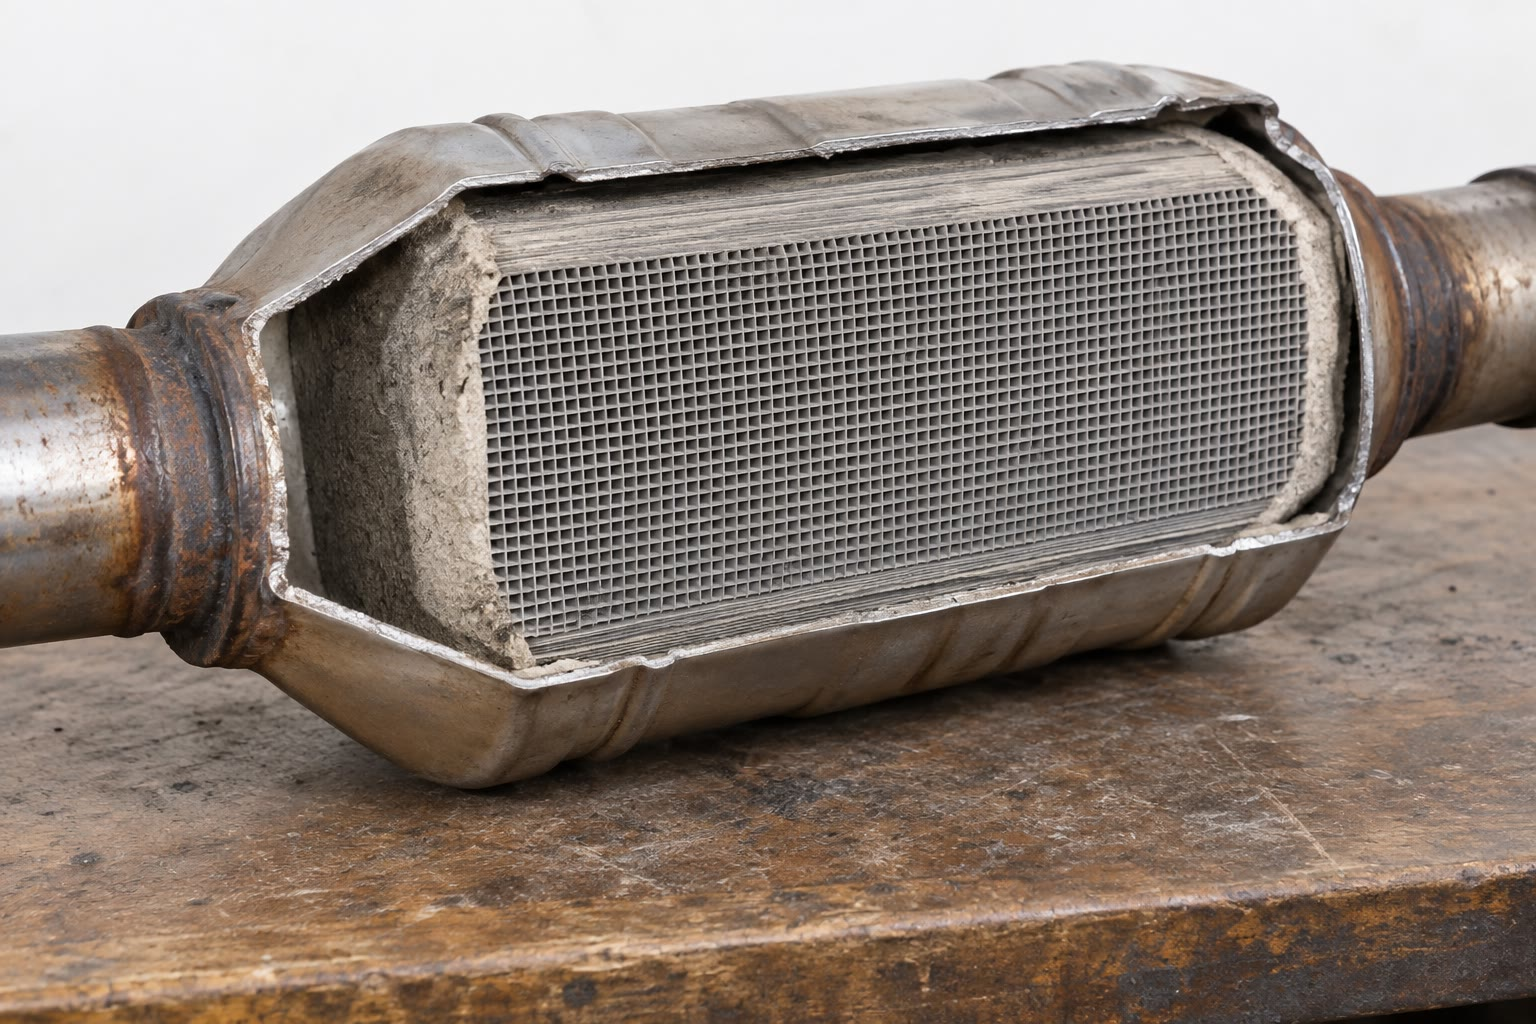
\includegraphics[width=0.45\linewidth]{images/book1/ai/g12-catalytic-converter.jpg}

{\small Un pot catalytique ouvert~: le cœur en nid d'abeilles.}
\end{omfigure}

\begin{history}[Haber, Bosch et l'ammoniac]
% ledger: haber:T, haber:p, nh3:world-2024
Au début du \textsc{xx}\textsuperscript{e}~siècle, le chimiste Fritz Haber trouva
comment combiner l'azote de l'\omterm{def:g4:air-a-mixture-of-gases:air}{air} avec l'hydrogène,
\ce{N2 + 3H2 -> 2NH3}, sur un \omterm{def:g12:catalysis:catalyst}{catalyseur} à base de fer, et l'ingénieur
Carl Bosch en fit un procédé industriel. Celui-ci fonctionne encore
aujourd'hui, entre 400
et \qty{500}{\celsius} et entre 150 et \qty{250}{atm}. En 2024, le monde
a produit de l'ammoniac contenant environ 150 millions de tonnes
d'azote, en majeure partie pour les engrais~: une grande part de l'azote
des aliments que nous mangeons est passée par un tel \omterm{def:g12:catalysis:catalyst}{catalyseur}.
\end{history}

\section{Les enzymes}

\begin{definition}[Enzyme]\label{def:g12:catalysis:enzyme}
Une \emph{enzyme}\index{enzyme} est une protéine fabriquée par un être
vivant, qui \omterm{def:g12:catalysis:catalyst}{catalyse} une réaction de sa chimie. Les enzymes sont très
efficaces et très spécifiques~: chacune ne convient qu'à quelques
\omterm{def:g7:atoms-and-molecules:molecule}{molécules}, et elles fonctionnent au mieux dans un domaine étroit de
température et d'acidité.
\end{definition}

\begin{example}[La catalase]\label{ex:g12:catalysis:catalase}
Le peroxyde d'hydrogène se forme dans les cellules comme sous-produit,
et il leur est nocif. La catalase, une \omterm{def:g12:catalysis:enzyme}{enzyme} présente dans le sang, le
foie et de nombreux tissus végétaux, le décompose en eau et en
dioxygène à une vitesse énorme~: c'est la mousse sur un genou écorché, ou
sur une tranche de pomme de terre crue. Une pomme de terre cuite à l'eau
ne donne pas de mousse~: la cuisson a détruit la forme de l'\omterm{def:g12:catalysis:enzyme}{enzyme}.
\end{example}

\begin{omfigure}
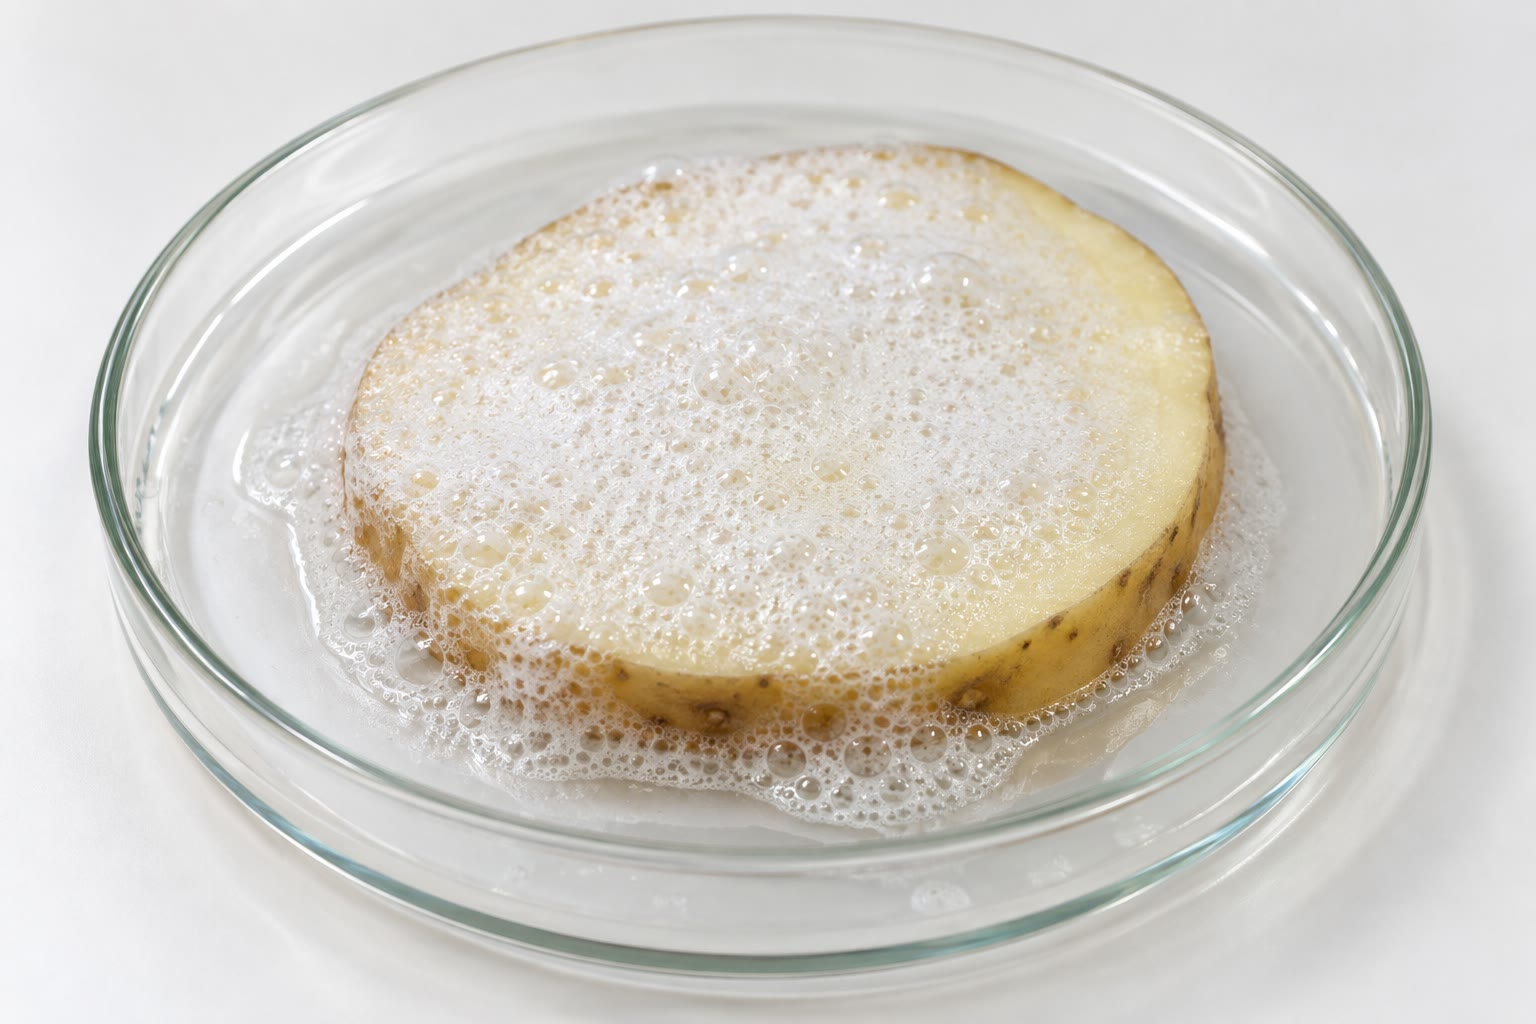
\includegraphics[width=0.45\linewidth]{images/book1/ai/g12-potato-peroxide.jpg}

{\small De l'eau oxygénée sur une tranche de pomme de terre crue~: la
catalase à l'œuvre.}
\end{omfigure}

\section{La sélectivité}

\begin{definition}[Catalyseur sélectif]\label{def:g12:catalysis:selective}
Quand les mêmes \omterm{def:g7:chemical-reactions:reactant}{réactifs} peuvent donner plusieurs réactions, un
\emph{catalyseur sélectif}\index{catalyseur selectif@catalyseur sélectif} accélère l'une
d'elles beaucoup plus que les autres, et décide ainsi des produits
formés.
\end{definition}

\begin{example}[Deux destins pour l'éthanol]\label{ex:g12:catalysis:ethanol}
De la vapeur d'éthanol chaude, passée sur de l'alumine, perd de l'eau et
donne de l'éthène, \ce{C2H5OH -> C2H4 + H2O} (une \omterm{def:g12:curly-arrows:categories}{élimination})~; passée
sur du cuivre chaud, elle perd du dihydrogène et donne de l'éthanal,
\ce{C2H5OH -> CH3CHO + H2}. Même \omterm{def:g7:chemical-reactions:reactant}{réactif}, deux \omterm{def:g12:catalysis:catalyst}{catalyseurs}, deux
produits.
\end{example}

\begin{remark}[L'industrie et le vivant fonctionnent grâce aux catalyseurs]\label{rem:g12:catalysis:everywhere}
La plupart des produits de l'industrie chimique, des carburants aux
\omterm{def:g8:plastics:plastic}{matières plastiques} et aux engrais, sont fabriqués à l'aide de
\omterm{def:g12:catalysis:catalyst}{catalyseurs}~; trouver un \omterm{def:g12:catalysis:catalyst}{catalyseur} plus actif ou plus sélectif
économise de l'énergie et réduit les déchets. Chaque réaction d'une
cellule vivante est catalysée par une \omterm{def:g12:catalysis:enzyme}{enzyme}.
\end{remark}

\begin{safety}{\ghs[0.82cm]{GHS03}\ghs[0.82cm]{GHS05}\ghs[0.82cm]{GHS07}}
% ledger: ghs:H2O2
Le peroxyde d'hydrogène concentré est un \omterm{def:g11:redox:oxidant}{oxydant} puissant qui peut
entretenir un incendie~; il brûle la peau et les yeux, et il est nocif
en cas d'ingestion. Les solutions diluées du laboratoire exigent malgré
tout lunettes et gants~; la décomposition libère du dioxygène, on ne la
réalise donc jamais dans un récipient fermé.
\end{safety}

\section{Exercices}


\begin{exercise}[$\star$]\label{exo:g12:catalysis:1}
Dans la décomposition du peroxyde d'hydrogène catalysée par les \omterm{def:g9:ions:ion}{ions}
iodure, quelles espèces sont des \omterm{def:g7:chemical-reactions:reactant}{réactifs}, lesquelles sont des produits,
laquelle est le \omterm{def:g12:catalysis:catalyst}{catalyseur}, laquelle est un intermédiaire~?
\end{exercise}

\begin{exercise}[$\star$]\label{exo:g12:catalysis:2}
\omterm{def:g12:catalysis:homogeneous}{Catalyse homogène} ou hétérogène~: des \omterm{def:g9:ions:ion}{ions} iodure dans de l'eau
oxygénée~; le platine d'un pot catalytique~; le fer de la \omterm{def:g10:synthesis-yield:synthesis}{synthèse} de
l'ammoniac~; des \omterm{def:g9:ions:ion}{ions} fer(III) dans de l'eau oxygénée~?
\end{exercise}

\begin{exercise}[$\star$]\label{exo:g12:catalysis:3}
Sur les profils énergétiques, quel chemin présente la barrière la plus
haute~? Les énergies de départ et d'arrivée sont-elles les mêmes sur les
deux chemins~? Qu'est-ce que cela signifie pour les produits~?
\end{exercise}

\begin{exercise}[$\star$]\label{exo:g12:catalysis:4}
Pourquoi un \omterm{def:g12:catalysis:catalyst}{catalyseur} n'apparaît-il pas dans l'équation globale d'une
réaction~?
\end{exercise}

\begin{exercise}[$\star$]\label{exo:g12:catalysis:5}
Pourquoi les \omterm{def:g12:catalysis:catalyst}{catalyseurs} solides de l'industrie sont-ils utilisés sous
forme de poudres fines ou de fines couches sur des supports poreux~?
\end{exercise}

\begin{exercise}[$\star\star$]\label{exo:g12:catalysis:6}
Additionner les deux étapes de la décomposition du peroxyde d'hydrogène
catalysée par les \omterm{def:g9:ions:ion}{ions} fer(III), et montrer que les \omterm{def:g9:ions:ion}{ions} fer et les \omterm{def:g9:ions:ion}{ions}
hydrogène s'éliminent.
\end{exercise}

\begin{exercise}[$\star\star$]\label{exo:g12:catalysis:7}
Lire les courbes du dioxygène dégagé. Combien de temps faut-il à chaque
expérience pour libérer la moitié du volume final~? Par quel facteur le
\omterm{def:g12:catalysis:catalyst}{catalyseur} raccourcit-il cette durée~?
\end{exercise}

\begin{exercise}[$\star\star$]\label{exo:g12:catalysis:8}
On n'utilise pas d'essence au plomb dans les voitures équipées d'un pot
catalytique~: le plomb se dépose sur le platine et y reste. Expliquer
pourquoi cela ruine le pot, bien que le platine ne soit pas consommé par
la réaction normale.
\end{exercise}

\begin{exercise}[$\star\star$]\label{exo:g12:catalysis:9}
Un élève mesure la mousse produite par des tranches de pomme de terre
dans de l'eau oxygénée à 10, 25, 37, 60 et \qty{80}{\celsius}~: la
mousse augmente jusque vers \qty{37}{\celsius}, puis diminue, et
disparaît presque à
\qty{80}{\celsius}. Expliquer les deux parties de la courbe.
\end{exercise}

\begin{exercise}[$\star\star$]\label{exo:g12:catalysis:10}
Écrire l'équation de la réaction entre le monoxyde de carbone et le
monoxyde d'azote dans un pot catalytique, et vérifier qu'elle est
ajustée. Pourquoi les deux polluants sont-ils éliminés en même temps~?
\end{exercise}

\begin{exercise}[$\star\star$]\label{exo:g12:catalysis:11}
\qty{10.0}{mL} d'eau oxygénée dégagent \qty{72}{mL} de dioxygène à
\qty{20}{\celsius} quand ils se décomposent entièrement. Calculer la
quantité de dioxygène ($V_m = \qty{24.1}{L/mol}$), puis la concentration
de la solution en peroxyde d'hydrogène.
\end{exercise}

\begin{exercise}[$\star\star\star$]\label{exo:g12:catalysis:12}
De la vapeur d'éthanol passée sur de l'alumine donne de l'éthène~;
passée sur du cuivre, elle donne de l'éthanal. Écrire les deux
équations, donner la catégorie de la première, et expliquer ce qu'est un
\omterm{def:g12:catalysis:selective}{catalyseur sélectif}.
\end{exercise}

\begin{exercise}[$\star\star\star$]\label{exo:g12:catalysis:13}
Un \omterm{def:g12:catalysis:catalyst}{catalyseur} rend une réaction dix fois plus rapide. Un élève affirme
qu'il donne aussi dix fois plus de produit. Corriger cette affirmation à
l'aide des courbes du dioxygène dégagé.
\end{exercise}

\begin{exercise}[$\star\star\star$]\label{exo:g12:catalysis:14}
Une \omterm{def:g7:atoms-and-molecules:molecule}{molécule} de catalase décompose quelques millions de \omterm{def:g7:atoms-and-molecules:molecule}{molécules} de
peroxyde d'hydrogène par seconde. En prenant $\num{5e6}$ par seconde,
combien de temps faut-il à une \omterm{def:g7:atoms-and-molecules:molecule}{molécule} d'\omterm{def:g12:catalysis:enzyme}{enzyme} pour décomposer une
\omterm{def:g10:the-mole:amount}{mole} de peroxyde d'hydrogène~? Combien de \omterm{def:g7:atoms-and-molecules:molecule}{molécules} d'\omterm{def:g12:catalysis:enzyme}{enzyme} le feraient
en une seconde~? (Calcul d'ordres de grandeur~; la vitesse est une
donnée de l'exercice.)
\end{exercise}

\begin{exercise}[$\star\star\star$]\label{exo:g12:catalysis:15}
% ledger: nh3:world-2024
Le monde a produit environ 150 millions de tonnes d'azote sous forme
d'ammoniac en 2024. Quelle masse d'ammoniac cela représente-t-il~?
Quelle quantité de diazote a été combinée~?
\end{exercise}

\section{Problème~: l'eau oxygénée du coiffeur}

\begin{problem}[{Problème du week-end --- quelle est la concentration
d'une eau oxygénée «~à 20 volumes~»~?}]
\label{pb:g12:catalysis:1}
% ledger: const:Vm1, ghs:H2O2, aw:H, aw:O
Les coiffeurs utilisent des solutions de peroxyde d'hydrogène dont le
titre est donné en «~volumes~»~: une eau oxygénée «~à 20 volumes~» est
une solution dont \qty{1}{L} dégage \qty{20}{L}
de dioxygène quand elle se décompose entièrement, le gaz étant mesuré à
\qty{0}{\celsius} et à la pression atmosphérique normale, conditions
dans lesquelles une \omterm{def:g10:the-mole:amount}{mole} de gaz occupe \qty{22.4}{L}.

\medskip
\noindent\textbf{Partie I --- La décomposition.}
\begin{enumerate}
  \item Écrire l'équation de la décomposition du peroxyde d'hydrogène.
  \item La décomposition est-elle une \omterm{def:g11:redox:reaction}{réaction d'oxydoréduction}~?
        Trouver l'\omterm{def:g11:redox:oxidant}{oxydant} et le \omterm{def:g11:redox:oxidant}{réducteur} (le peroxyde d'hydrogène est
        les deux à la fois).
  \item Pourquoi un flacon se conserve-t-il des mois, alors que la
        réaction est possible~?
\end{enumerate}

\medskip
\noindent\textbf{Partie II --- Ce que signifie «~20 volumes~».}
\begin{enumerate}[resume]
  \item Quelle quantité de dioxygène \qty{1}{L} de solution dégage-t-il~?
  \item En déduire la quantité de peroxyde d'hydrogène dans \qty{1}{L}.
  \item Donner la \omterm{def:g10:concentration-and-dilution:molar-concentration}{concentration molaire}.
  \item Calculer la \omterm{def:g10:the-mole:molar-mass}{masse molaire} du peroxyde d'hydrogène et la
        \omterm{def:g10:concentration-and-dilution:mass-concentration}{concentration massique}.
  \item Que signifierait «~10 volumes~» en \omterm{def:g10:the-mole:amount}{moles} par litre~?
\end{enumerate}

\medskip
\noindent\textbf{Partie III --- Deux \omterm{def:g12:catalysis:catalyst}{catalyseurs}.}
\begin{enumerate}[resume]
  \item On ajoute à un échantillon une goutte de sang (catalase), et à
        un autre quelques gouttes de chlorure de fer(III). De quelle
        \omterm{def:g12:catalysis:catalyst}{catalyse} s'agit-il dans chaque cas~?
  \item Écrire les deux étapes de la \omterm{def:g12:catalysis:catalyst}{catalyse} par les \omterm{def:g9:ions:ion}{ions} fer(III) et
        vérifier que leur somme est la décomposition.
  \item À l'aide des courbes du dioxygène dégagé, décrire comment le
        volume de dioxygène évolue avec et sans \omterm{def:g12:catalysis:catalyst}{catalyseur}, et ce qui
        reste identique.
  \item Pourquoi la couleur d'un échantillon catalysé par les \omterm{def:g9:ions:ion}{ions}
        fer(III) change-t-elle pendant la réaction et revient-elle à la
        fin~?
  \item Pourquoi une pomme de terre cuite ne fait-elle pas mousser la
        solution~?
\end{enumerate}

\medskip
\noindent\textbf{Partie IV --- Le flacon.}
\begin{enumerate}[resume]
  \item Quel volume de dioxygène, mesuré à \qty{0}{\celsius}, un flacon
        de \qty{100}{mL} peut-il dégager~?
  \item Quel volume cela représente-t-il à \qty{20}{\celsius} ($V_m =
        \qty{24.1}{L/mol}$)~?
  \item Pourquoi le bouchon d'un tel flacon doit-il laisser le gaz
        s'échapper lentement~?
  \item Un flacon conservé longtemps est titré~: on trouve
        \qty{1.50}{mol/L}. À combien de «~volumes~» cela correspond-il
        maintenant~?
  \item Quelle fraction du peroxyde d'hydrogène s'est décomposée~?
  \item Donner la réponse finale~: quelle est la \omterm{def:g10:concentration-and-dilution:molar-concentration}{concentration molaire}
        d'une eau oxygénée «~à 20 volumes~»~?
\end{enumerate}
\end{problem}
